\section{logarithmic wind law}
From the log-wind law we know
\begin{equation}
    \mathbf{u} = \frac{u_*}{k}\\ln\left( \frac{z}{z_0}\right) \implies \derivate{\mathbf{u}}{z} = \frac{u_*}{kz}
\end{equation}
However we also know from Prandtl that  
\begin{equation}
    K_m = l^2 \abs{\derivate{\mathbf{u}}{z}}
\end{equation}
using these two relations we get together with the assumption that $l=kz$ we obtain
\begin{equation}
    K_m = (kz)^2 \frac{u_*}{kz} = ku_*z
\end{equation}
This $K_m$ is the turbulent viscosity in the boundary layer. However, we know that this should start to decay after a certain height, and one can thus assume decay so that the total kinematic viscosity is zero at height $z=H$ as:
\begin{equation}
    \nu = ku_*z\left(1-\frac{z}{H}\right)
\end{equation}
or one could expect a exponential decay at as 
\begin{equation}
    \nu = ku_*ze^z/H
\end{equation}

\begin{figure}[H]
    \centering    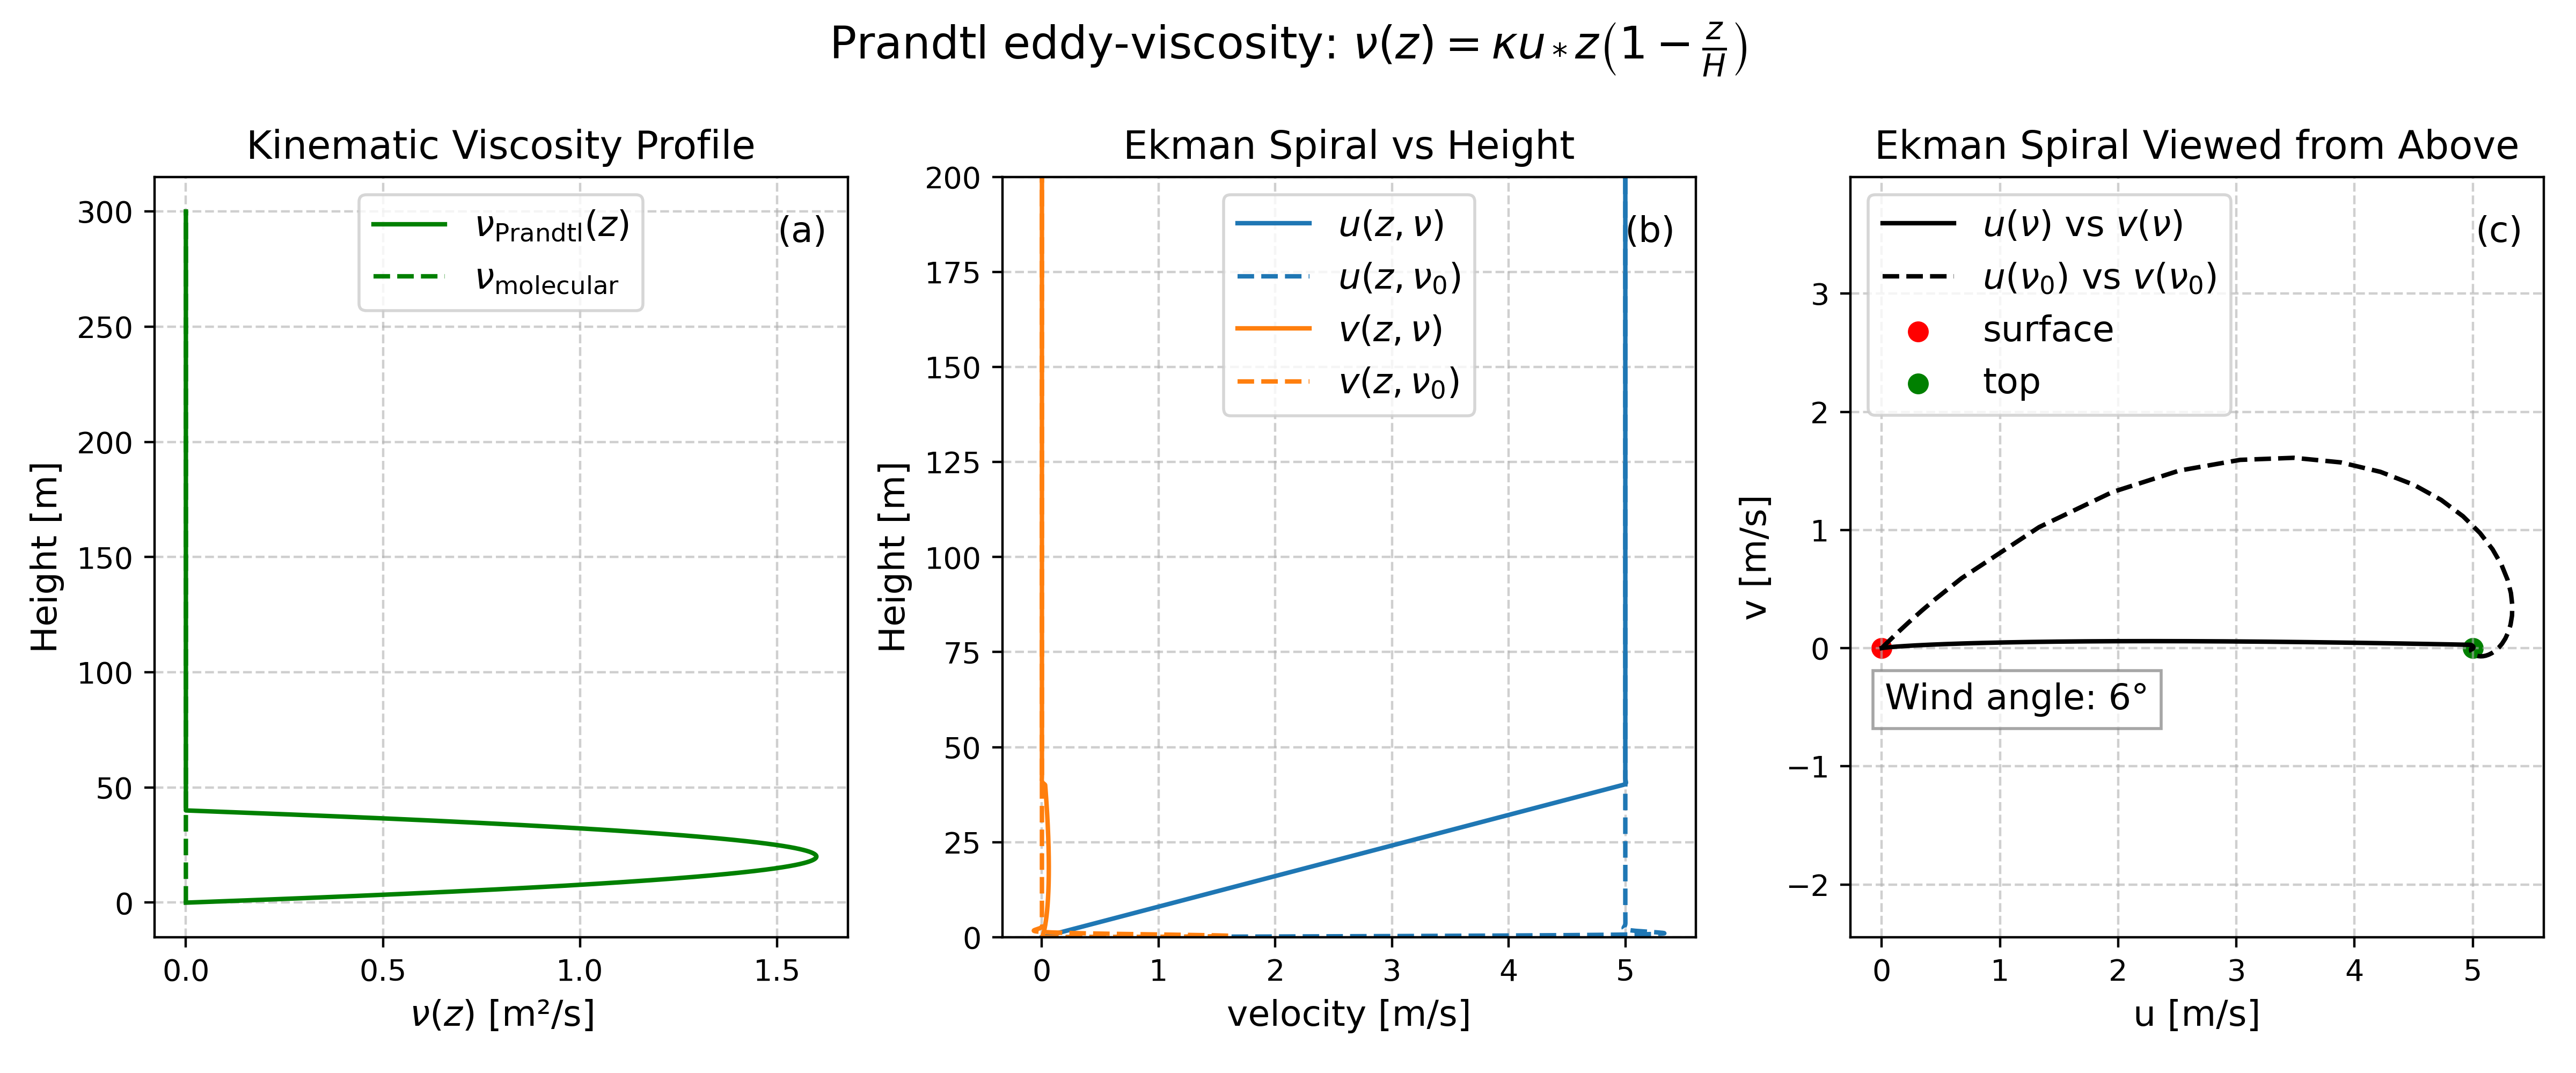
\includegraphics[width=0.9\textwidth]{Figures/BVP_Prandtl1.png}
    \caption{This figure shows the numeric solution for another specific profile.}
    \label{fig:numeric_Prandtl1}
\end{figure}

\begin{figure}[H]
    \centering    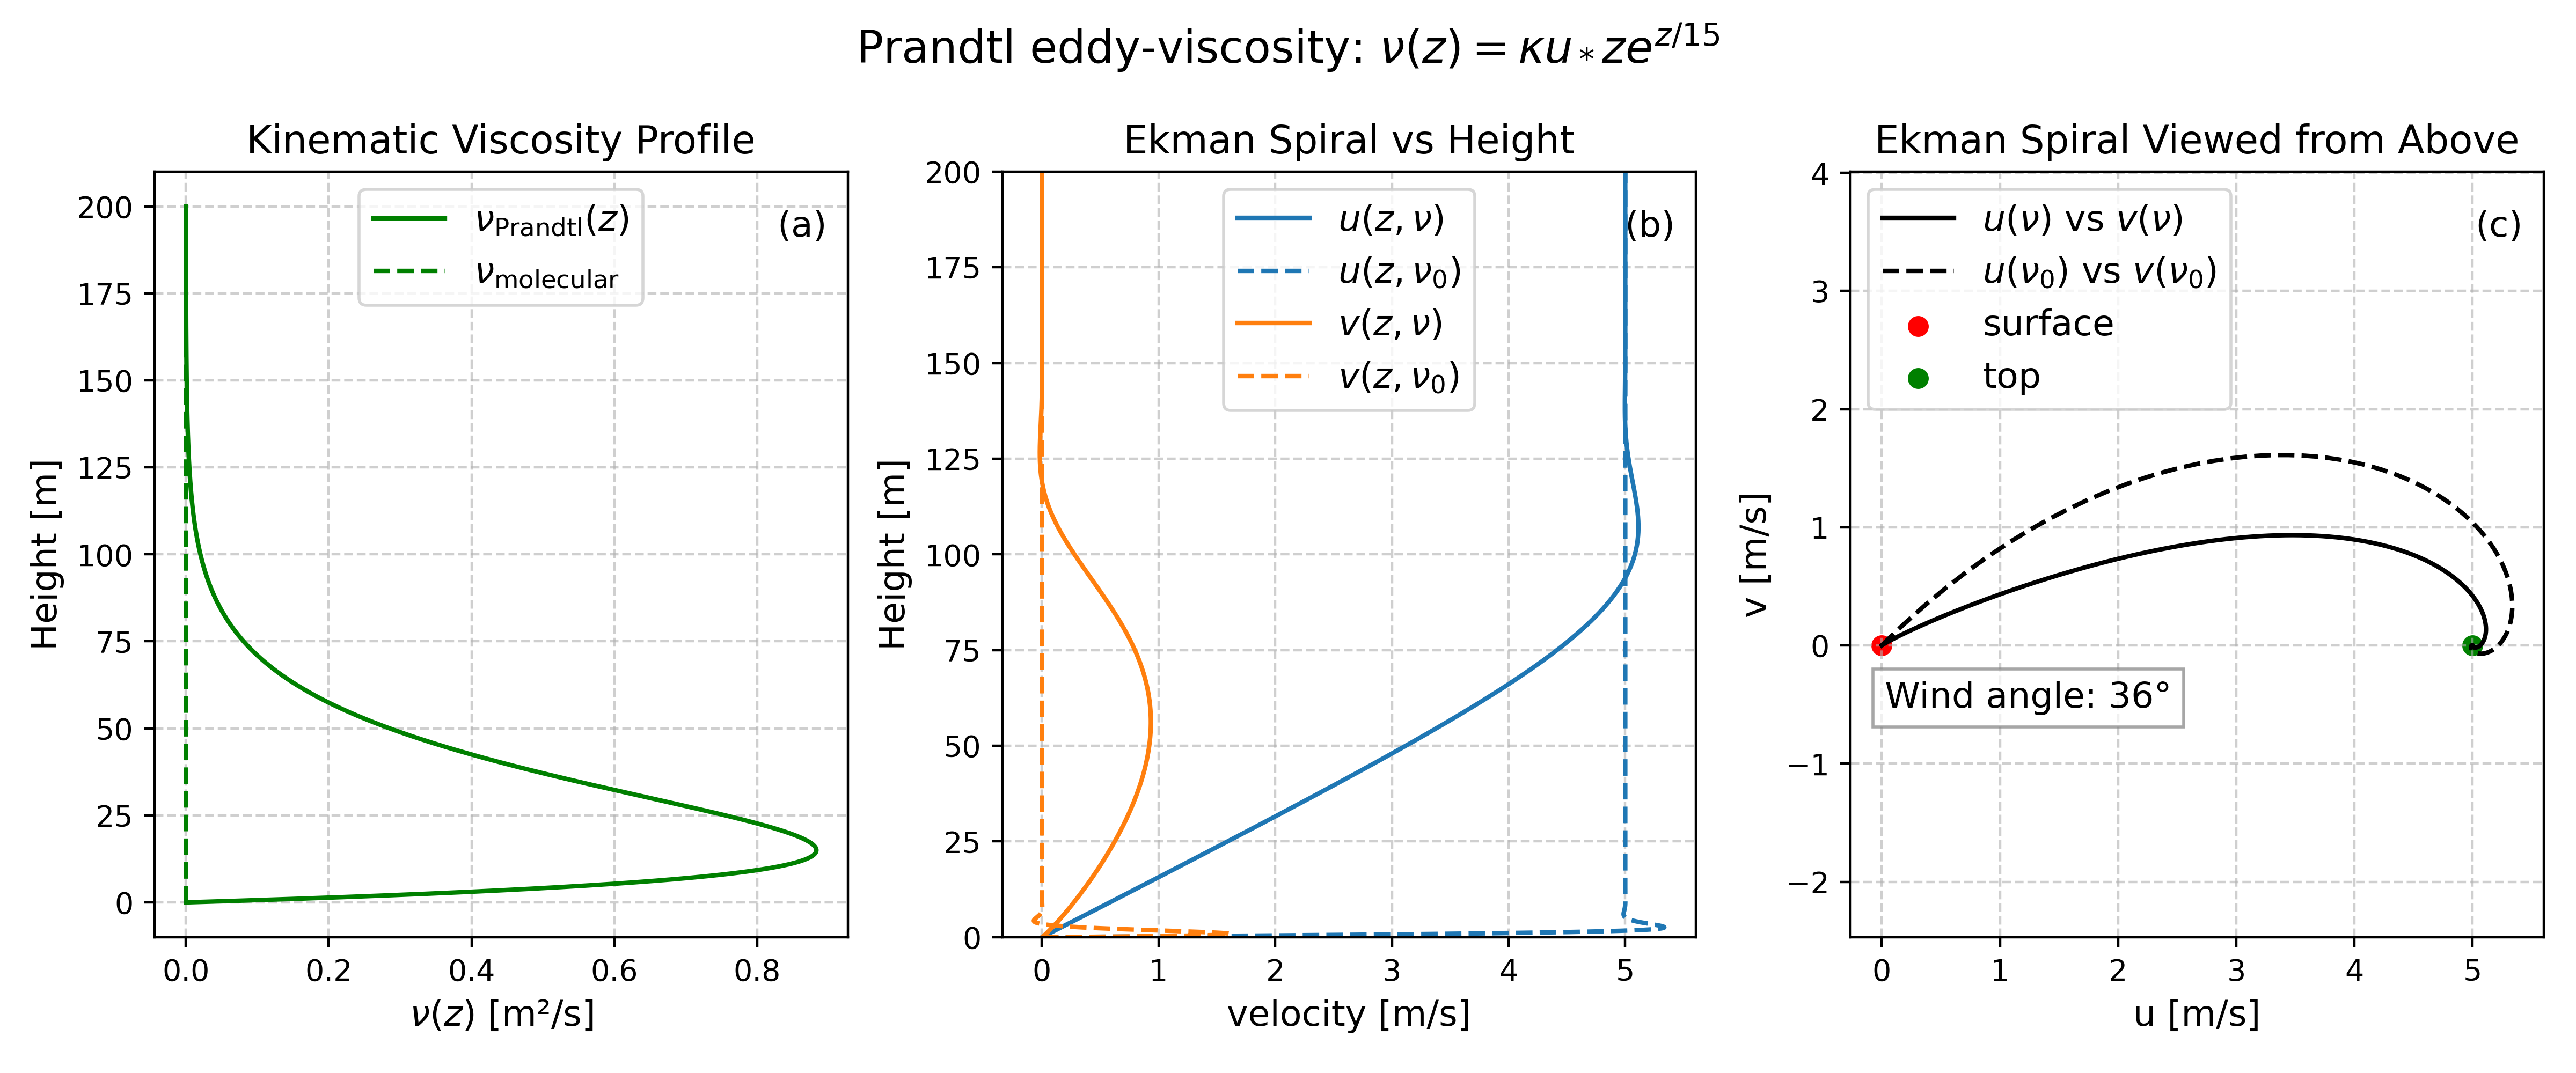
\includegraphics[width=0.9\textwidth]{Figures/BVP_Prandtl2.png}
    \caption{This figure shows the numeric solution for another, more realistic, profile.}
    \label{fig:numeric_Prandtl2}
\end{figure}

$\mathbf{1}$